\documentclass[letterpaper, 12pt]{article}
\usepackage[round]{natbib}
\bibliographystyle{apalike}
\usepackage[margin=1in]{geometry}
\usepackage{enumitem}
\usepackage{csquotes}
\usepackage{graphicx}
\usepackage{float}
\usepackage{svg}


\usepackage{xcolor} % 
\newcommand{\bca}[1]{\textcolor{blue}{BA: #1}} % Blair
\newcommand{\jl}[1]{\textcolor{purple}{JL: #1}} % Li
\newcommand{\todo}[1]{\textcolor{red}{#1}} % Things to fix.

\begin{document}
%\title{Proposal for the application to UTSC Postdoctoral Fellowship %Program}
%\author{Jiangtian Li}
%\maketitle


A central challenge in developing a theory of how the mind processes language is how the meanings of ambiguous words are resolved. Approximately 85\% of the words in the world's languages are ambiguous, yet in the vast majority of circumstances, humans resolve this ambiguity correctly and effortlessly \citep{KleinRepresentationPolysemousWords2001}.  For example, in the phrase ``A prime minister wields significant power'' a reader has no difficulty evoking a ``political power'' interpretation as opposed to an ``electrical power'' interpretation.  However, how ambiguity is resolved remains open, despite having received attention from interdisciplinary researchers (including philosophers such as myself, as well as linguists, and psychologists), and despite the game-changing role that a theory of ambiguity resolution could have for artificial intelligence. Indeed, a firm grasp of the fundamental principles governing ambiguity resolution are likely to revolutionize applications of language technologies including building better ``bots'' to communicate with customers online, and better automated screening of user content for remarks that are inappropriate or discriminatory.  

My proposal builds upon the latest insights from several disciplines to develop and test a novel account of ambiguity resolution. First, my philosophy background makes me appreciate the fundamental weakness of a cognitive system without grounded and referential information connected to the outer world \citep{harnadSymbolGroundingProblem1990, searleMindsBrainsPrograms1980}. Second, I will adopt the view in cognitive science that understanding language fundamentally requires language to be part of a broader system for understanding and communicating about situations. Third, from the psycholinguistics and neuroscience literatures (including work by my proposed advisor, Professor Blair Armstrong), I will draw on recent findings demonstrating how building in additional neurobiological plausibility into simulations are essential for simulating a number of aspects of ambiguity resolution \citep{Armstrong2016Disparatesemanticambiguity}.

RESEARCH PLAN: My research plan starts from a (relatively) simple neural network model and gradually increasing the complexity of this model to achieve better performance. It quantifies how each new level of complexity improves over simpler models. Such complexity is not achievable until the recent development in training methods and hardwares. All of these models will be trained on databases of images and their associated captions, such as the COCO (Common Objects in Context) dataset, so that they, except the first model, learn to see objects while simultaneously processing their verbal description. And each model will be tested against published data in the psycholinguistics literature which will serve as the ``gold standard'' for successfully modeling human ambiguity resolution abilities.


1.  Language-only model. The first model will be trained only on the verbal input in the COCO dataset, and provides a baseline for how much disambiguating information can be extracted from text alone.  This approach is currently widespread in computational linguistics, and has been shown to contain substantial (although far from complete) disambiguating information. \citep{beekhuizenWhatCompanySemantically2018}

2.  Integrated vision-and-language model.  The second model will add a visual processing system to the model developed in (1), and will serve as a first validation for how visual information can provide additional constraint on word meaning than the prior model.

3.  More biologically plausible integrated model.  The third model will focus on how several key principles from cognitive and systems neuroscience could further enhance performance in the model: 3(a) Addition of an attention mechanism. Humans do not process all of the information their eyes take in equally well, rather, they focus attention on one part of the visual field and extract substantially more information from that area than others. 3(b) More realistic cortical connectivity.  In artificial neural networks, artificial neurons are typically able to send both positive (excitatory) and negative (inhibitory) information to other neurons, and often every neuron in one simulated brain area is connected to every neuron in another brain area.  In ``real'' neural networks, such as the human brain, neurons send excitatory OR inhibitory information, NOT both; there are vastly more ($\approx85\%$) excitatory neurons than inhibitory neurons ($\approx15\%$), and there are relatively few connections between different brain regions, such as vision and language. Prior work \citep{laszloPSPsERPsApplying2014, Armstrong2016Disparatesemanticambiguity} has established that these principles critically shape what type of information shapes network performance, including word disambiguation. 

EXPECTED OUTCOME AND IMPLICATIONS: I will revolutionize how ambiguity is thought about in many fields by merging insights from several fields to develop an account that would not emerge from any one discipline in isolation. Another implication is how abstract polysemous words are understood based on visual information. The political and ability senses of power are less connected to the physical world but people have been arguing that they share the same root as more physical words. This project will also serve as an attempt to test where the meanings of abstract polysemous words are rooted. Finally, the project can be potentially patented, if successful, to allow its free use to academics as well as its incorporation into industry, like Microsoft, Facebook, Google, etc.

\begin{figure}[h]
\begin{center}
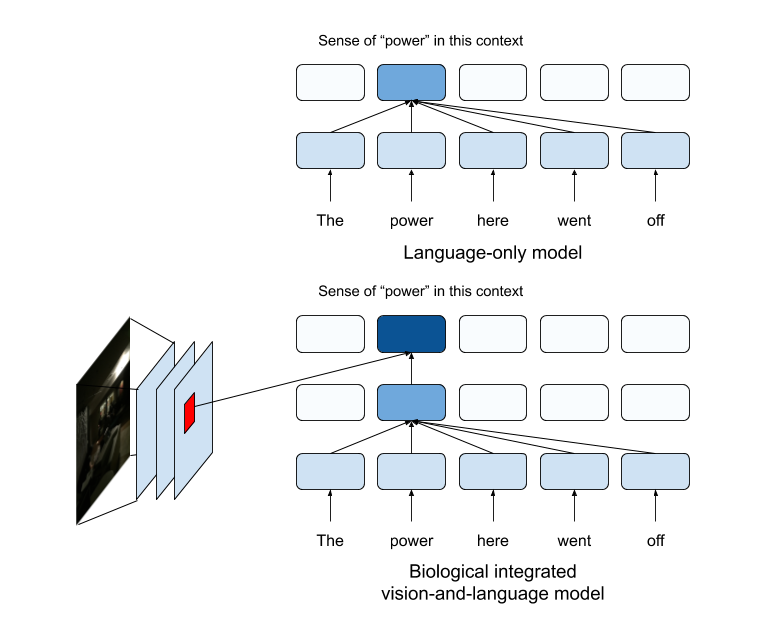
\includegraphics[width=0.7\textwidth,keepaspectratio]{model_figure}
\end{center}
    \caption{Computational models that are going to be build in this project.}
\end{figure}

\newpage
% \bibliography{/Users/jiangtianli/MyWriting/Mybib.bib}
\bibliography{Proposal_for_fellowship.bib}
\end{document}
